% If you do want an image in the colophon:
\begin{figure}
  \vspace{50pt}
  \centering
    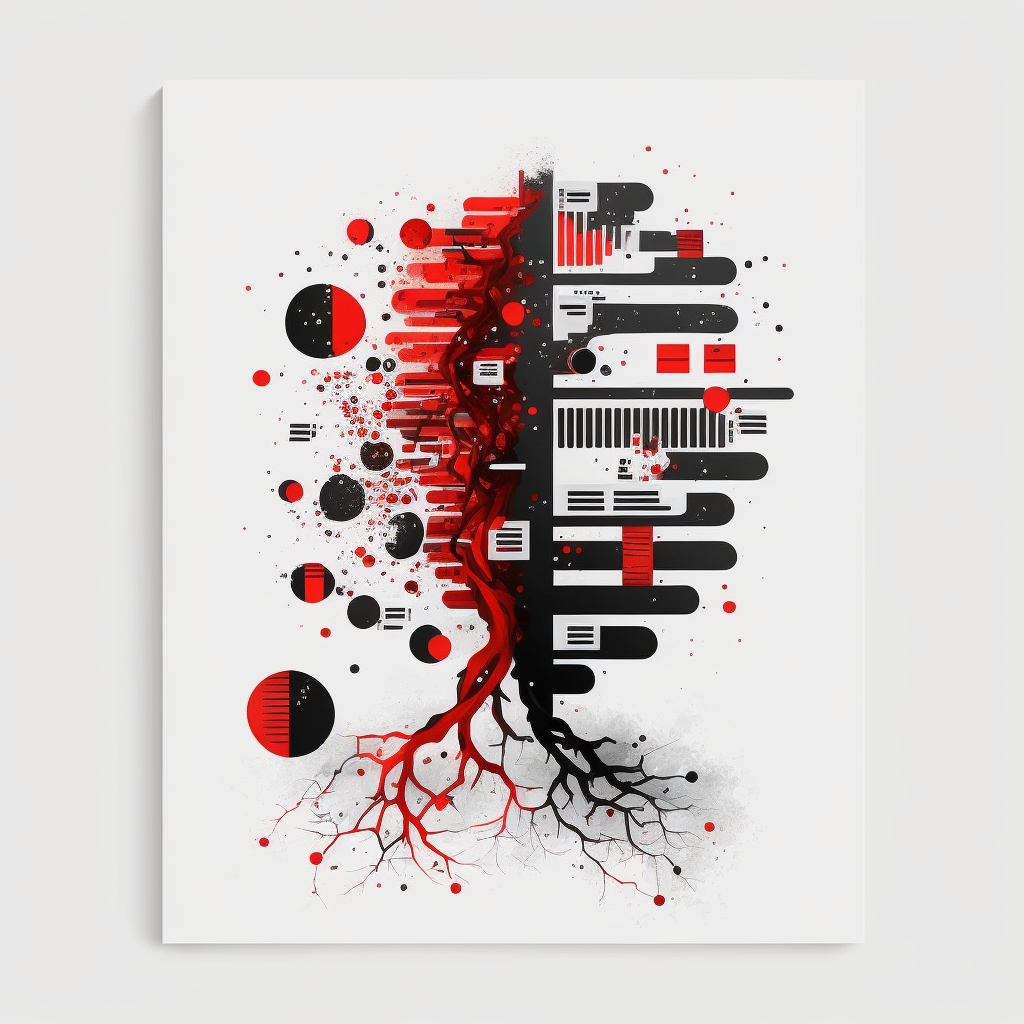
\includegraphics[width=180pt]{endmatter/colophon.png}
\end{figure}

% If you don't want an image in the colophon:
% \vspace*{200pt}

\begin{center}
\parbox{200pt}{\lettrine[lines=3,slope=-2pt,nindent=-4pt]{\textcolor{SchoolColor}{T}}{his thesis was typeset} using \LaTeX, originally developed by Leslie Lamport and based on Donald Knuth's \TeX. The body text is set in 11 point Egenolff-Berner Garamond, a revival of Claude Garamont's humanist typeface. Unless otherwise noted, illustrations found throughout this book were created by Helena and the MidJourney AI art assistant. The above image was prompted with ``the combination of an AI artificial intelligence and teaching and dna and science and cancer, minimalist aesthetic white background, black and red --v 4'' in MidJourney. The cover was designed by the amazing Saskia Hiltemann and myself.

\ \\
Hint for the puzzles on the back cover: esoteric languages. }
\end{center}
